\clearpage
%===================================================================================
\section{ATLAS and CMS results included in the database update}
%===================================================================================


%-----------------------------------------------------------------------------------------------
\subsection{ATLAS Run~2 results for 36~fb$^{-1}$}
%-----------------------------------------------------------------------------------------------

The ATLAS Run~2 results included in this release are summarised in Table~\ref{tab:ATLASresults} and explained in more detail below.

\begin{table}[h]\centering
\begin{tabular}{l | ccccccc}
mode & $\gamma\gamma$ & $ZZ^*$ & $WW^*$ & $\tau\tau$ & $b\bar b$ & inv. \\
\hline
ggH & \cite{Aaboud:2018xdt} & \cite{Aaboud:2017vzb} & \cite{Aaboud:2018jqu} & \cite{Aaboud:2018pen} & -- & --\\
VBF &  \cite{Aaboud:2018xdt} & \cite{Aaboud:2017vzb} & \cite{Aaboud:2018jqu} & \cite{Aaboud:2018pen} & \cite{Aaboud:2018gay} & -- \\
WH & \multirow{2}{*}{\!\!\cite{Aaboud:2018xdt}} & \multirow{2}{*}{\!\!\cite{Aaboud:2017vzb}} & -- & -- & \cite{Aaboud:2017xsd} & -- \\
ZH &  &  & -- & -- & \cite{Aaboud:2017xsd} & \cite{Aaboud:2017bja} \\
ttH & \cite{Aaboud:2018xdt,Aaboud:2017jvq} & \cite{Aaboud:2017vzb,Aaboud:2017jvq} & \cite{Aaboud:2017jvq} & \cite{Aaboud:2017jvq} & \cite{Aaboud:2017jvq,Aaboud:2017rss} & -- \\ 
\end{tabular}
\caption{Overview of ATLAS Run~2 results included in this release.} 
\label{tab:ATLASresults}
\end{table}

{\bf\boldmath $H\to\gamma\gamma$ (HIGG-2016-21):}  
The ATLAS analysis \cite{Aaboud:2018xdt} provides in Fig.~12 $H\to\gamma\gamma$ signal strengths separated into   
ggH, VBF, VH and ``top'' (ttH+tH) production modes. Since no correlations are given for the signal strengths, we 
use instead the correlations for the stage-0 simplified template cross sections (STXS) provided in Fig.~40a of the ATLAS 
paper, which should be a close enough match. It turns out that these data do not allow to reproduce very well the 
ATLAS coupling fits for $(C_V,\;C_F)$ or $(C_\gamma,\;C_g)$. The reason seems to be that the $\mu$ values 
rounded to one decimal are not  precise enough. We have therefore extracted the best-fit points and uncertainties 
from fits to the 1D profile likelihoods, which are provided as Auxiliary Figures 23a--d on the analysis webpage. 
and used these together with the STXS correlations in the {\tt Lilith} XML file. This gives a better coupling fit, as shown 
in the validation plots in Fig.~\ref{fig:validation_atlas_gamgam}. 

\begin{figure}[bh!]\centering
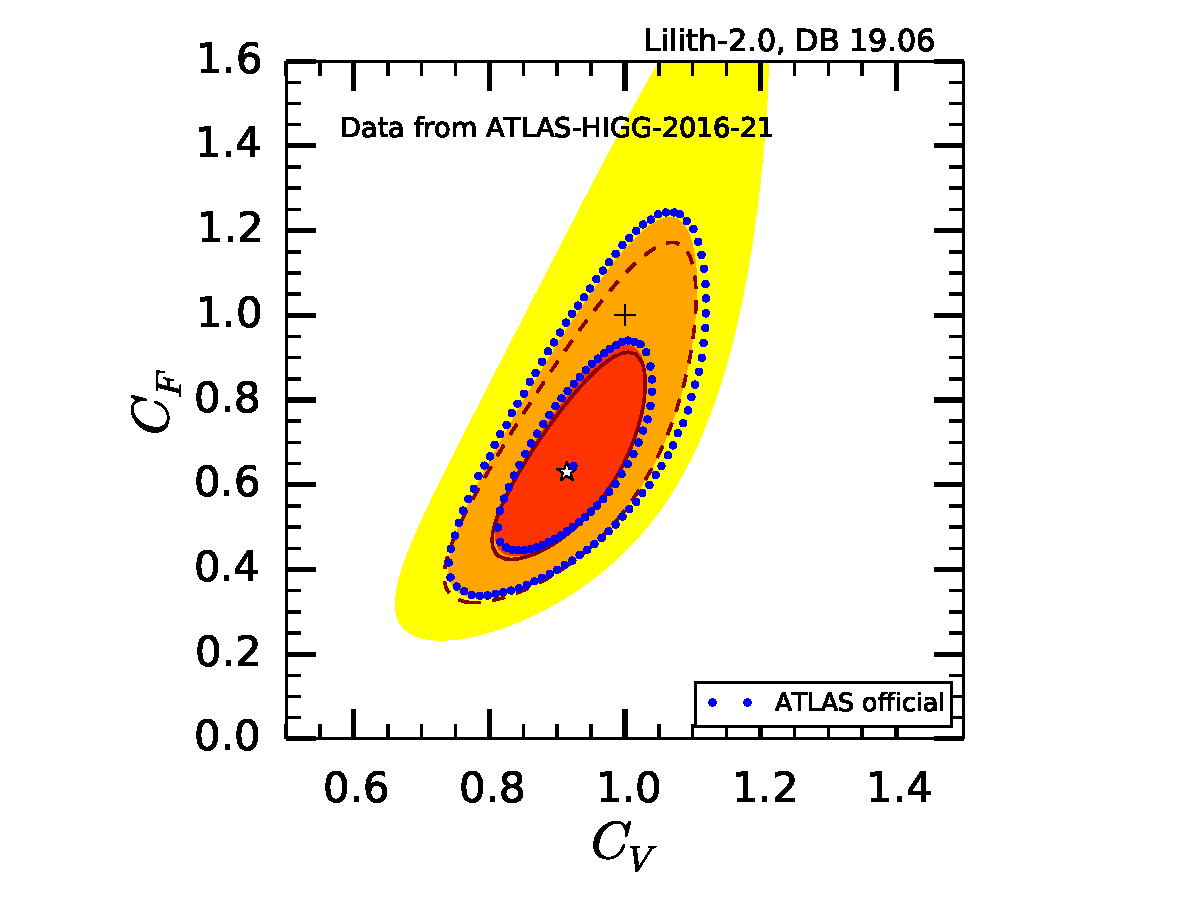
\includegraphics[width=0.5\textwidth]{validation/ATLAS/HIGG-2016-21-CVCF.pdf}%
\hspace{-12mm}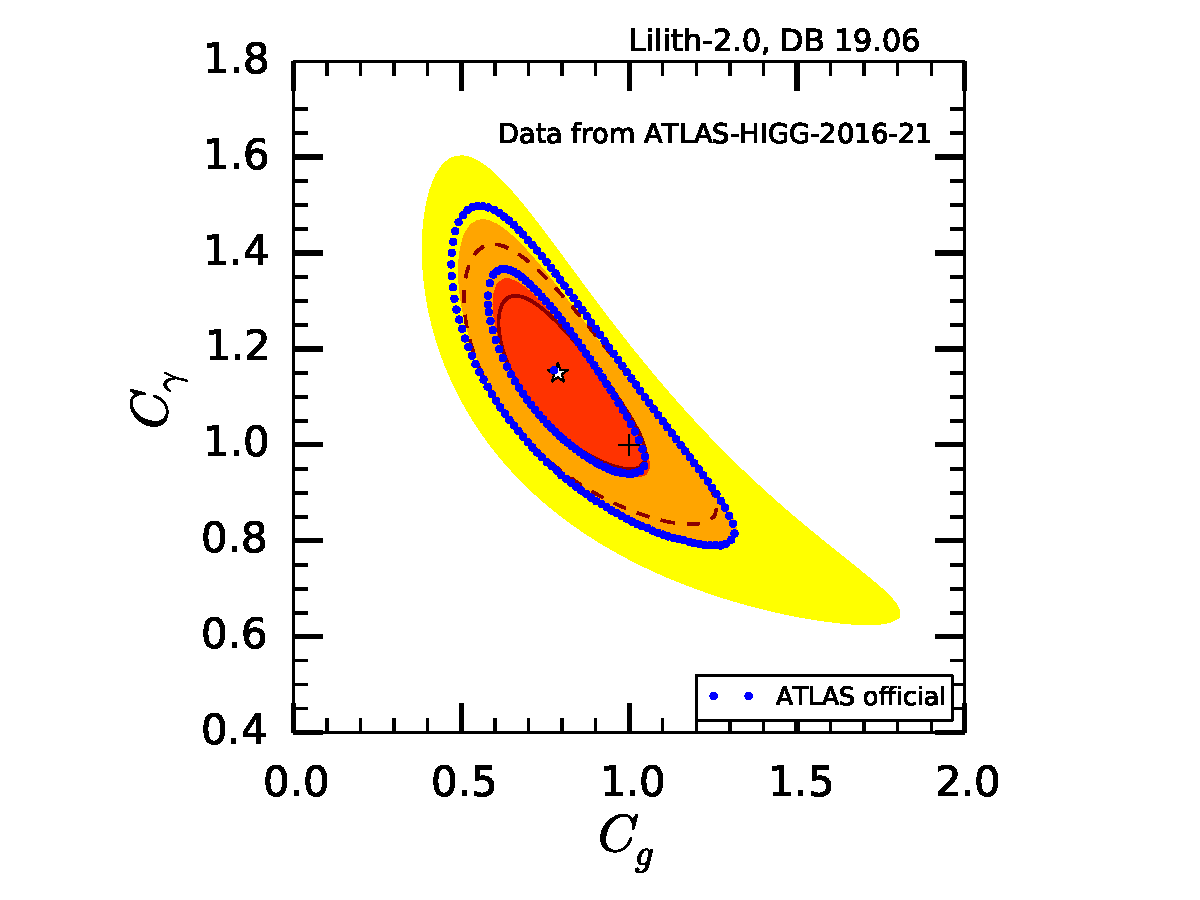
\includegraphics[width=0.5\textwidth]{validation/ATLAS/HIGG-2016-21-CgCGa.pdf}
\caption{Fit of $C_F$ vs.\ $C_V$ (left) and $C_\gamma$ vs.\ $C_g$ (right) for data from the ATLAS $H\to\gamma\gamma$ analysis~\cite{Sirunyan:2018koj}. The red, orange and yellow filled areas show the 
$68\%$,  $95\%$ and $99.7\%$ CL regions obtained with {\tt Lilith} using best-fit values and uncertainties for the signal strengths 
as extracted from Aux.\ Figs.~23a--d of the ATLAS analysis together with the correlation matrix for the stage-0 STXS. 
This can be compared to the $68\%$,  $95\%$ CL contours obtained using the rounded values from Fig.~12 of \cite{Sirunyan:2018koj} 
(solid and dashed dark red lines) and to the official $68\%$,  $95\%$ CL contours from ATLAS (blue dots).}
\label{fig:validation_atlas_gamgam}
\end{figure}
 
We note that the same fit quality is obtained when using only the correlation between ggH and VBF production modes 
(as 2D data) and treating VH and ttH as independent (as 1D data). The relevant XML files are all included in the 
database, so the user can choose the preferred combination. This is relevant to avoid double counting 
when combining this with other measurements, concretely with the data from~\cite{Aaboud:2017jvq}. \\

{\bf\boldmath $H\to ZZ^*\to 4l$ (HIGG-2016-22):} A similar issue as discussed for $H\to\gamma\gamma$ above arises 
when using the signal strengths given in Table~9 of \cite{Aaboud:2017vzb} together with the correlation matrix given in 
Aux.\ Fig.~4a. We therefore use $\mu({\rm ggH},\,ZZ^*)$ and $\mu({\rm VBF},\,ZZ^*)$ extracted from the 1D profile 
likelihoods Aux.\ Figs.~7a and 7b with a correlation $\rho=-0.41$ according to Aux.\ Fig.~4c. For the VH and ttH production 
modes, we convert the given 95\%~CL limits into $\mu({\rm VH},\,ZZ^*)=0^{+1.85}_{-0.0}$ and 
$\mu({\rm ttH},\,ZZ^*)=0^{+3.75}_{-0.0}$. For validation, we compare to the $C_F$ vs.\ $C_V$ fit from ATLAS, 
see Fig.~\ref{fig:validation_atlas_ZZ}.\\

\begin{figure}[htb!]\centering
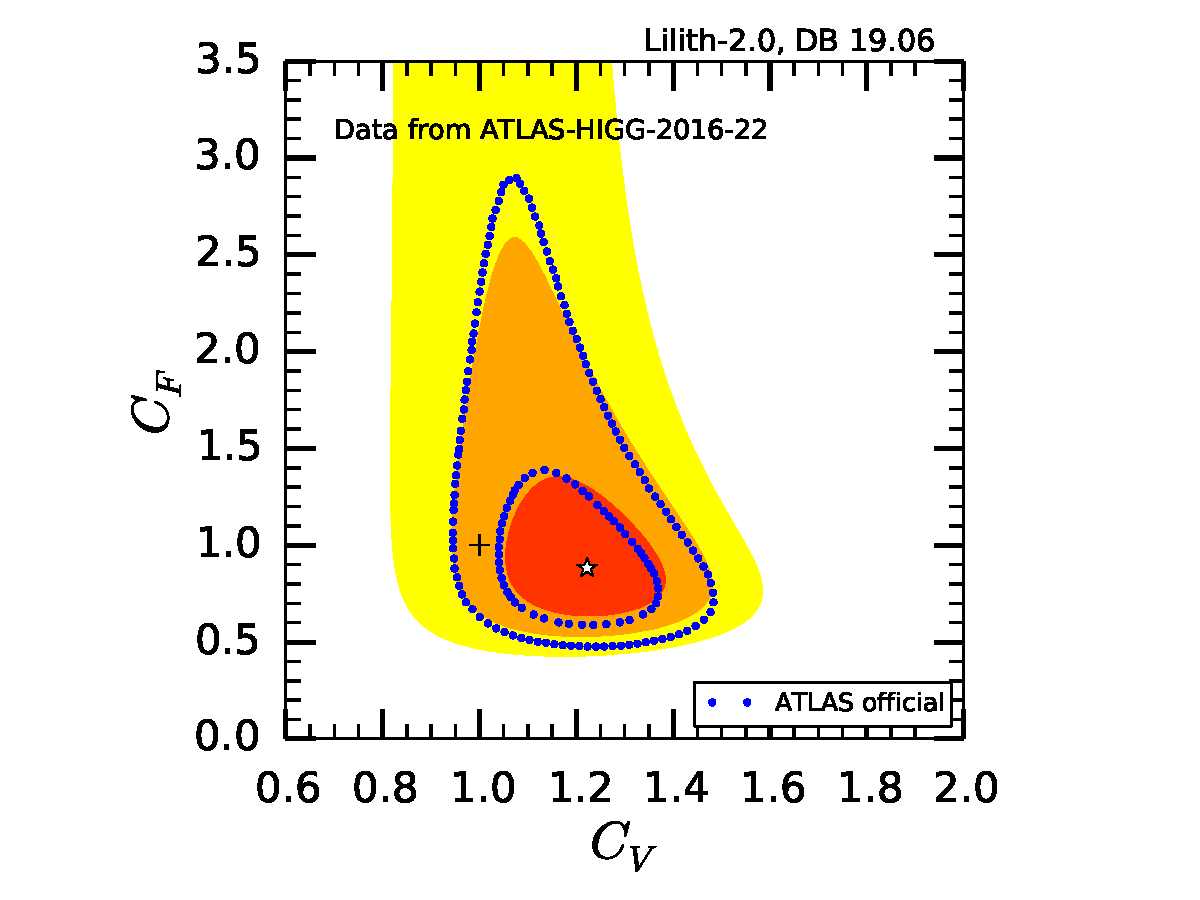
\includegraphics[width=0.5\textwidth]{validation/ATLAS/HIGG-2016-22-CVCF.pdf}
\caption{Fit of $C_F$ vs.\ $C_V$ for data from the ATLAS $H\to ZZ^*$ analysis~\cite{Aaboud:2017vzb}. 
The  $68\%$,  $95\%$ and $99.7\%$~CL regions obtained with {\tt Lilith} are shown as red, orange and yellow areas, 
and compared to the $68\%$,  $95\%$~CL contours from ATLAS (in blue).}
\label{fig:validation_atlas_ZZ}
\end{figure}


{\bf\boldmath $H\to WW^*\to 2l2\nu$ (HIGG-2016-07):} \\

{\bf\boldmath $H\to \tau\tau$ (HIGG-2017-07):} \\

{\bf\boldmath $H\to b\bar b$ (HIGG-2016-29 and HIGG-2016-30):}\\



{\bf\boldmath $H\to$~invisible (HIGG-2016-28):}
Results from the search for invisibly decaying Higgs bosons produced in association with a $Z$ boson are presented in \cite{Aaboud:2017bja}. Assuming the Standard Model $ZH$ production cross-section, an observed (expected) upper limit of 67\% (39\%) at the 95\% confidence level is set on BR$(H\to inv)$ for $m_H= 125$~GeV. We use $1-{\rm CLs}$ as function BR$(H\to inv)$ extracted from auxiliary Figure~1c on the analysis' webpage. 


\clearpage
%-----------------------------------------------------------------------------------------------
\subsection{CMS Run~2 results for 36~fb$^{-1}$}
%-----------------------------------------------------------------------------------------------

The CMS Run~2 results included in this release are summarised in Table~\ref{tab:CMSresults} and explained in more detail below.

\begin{table}[h]\centering
\begin{tabular}{l | ccccccc}
mode & $\gamma\gamma$ & $ZZ^*$ & $WW^*$ & $\tau\tau$ & $b\bar b$ & $\mu\mu$ & inv. \\
\hline
ggH & \cite{Sirunyan:2018koj} & \cite{Sirunyan:2018koj} & \cite{Sirunyan:2018koj} & \cite{Sirunyan:2018koj} & \cite{Sirunyan:2018koj} & \cite{Sirunyan:2018koj} & \cite{Sirunyan:2018owy} \\
VBF &  \cite{Sirunyan:2018koj} & \cite{Sirunyan:2018koj} & \cite{Sirunyan:2018koj} & \cite{Sirunyan:2018koj} &-- & \cite{Sirunyan:2018koj} & \cite{Sirunyan:2018owy} \\
WH &  \cite{Sirunyan:2018koj} & \cite{Sirunyan:2018koj} & \cite{Sirunyan:2018koj} & \cite{Sirunyan:2018cpi} & \cite{Sirunyan:2018koj} & -- & \cite{Sirunyan:2018owy} \\
ZH & \cite{Sirunyan:2018koj} & \cite{Sirunyan:2018koj} & \cite{Sirunyan:2018koj} & \cite{Sirunyan:2018cpi} & \cite{Sirunyan:2018koj} & -- & \cite{Sirunyan:2018owy} \\
ttH & \cite{Sirunyan:2018koj} & \cite{Sirunyan:2018koj} & \cite{Sirunyan:2018koj} & \cite{Sirunyan:2018koj} & \cite{Sirunyan:2018koj} & -- & -- \\
\end{tabular}
\caption{Overview of CMS Run~2 results included in this release. Note that we use the full $24\times 24$ correlation matrix 
for the signal strengths for each production and decay mode combination provided in \cite{Sirunyan:2018koj}.}
\label{tab:CMSresults}
\end{table}


{\bf\boldmath Combined measurements (HIG-17-031):} 
CMS presented in \cite{Sirunyan:2018koj} a combination of the individual measurements for the 
$H\to \gamma\gamma$~\cite{Sirunyan:2018ouh}, $ZZ$~\cite{Sirunyan:2017exp}, $WW$~\cite{Sirunyan:2018egh}, 
$\tau\tau$~\cite{Sirunyan:2017khh}, $b\bar b$~\cite{Sirunyan:2017elk,Sirunyan:2017dgc} and $\mu\mu$~\cite{Sirunyan:2018hbu} 
decay modes as well as the $t\bar tH$ analyses~\cite{Sirunyan:2018shy,Sirunyan:2018mvw,Sirunyan:2018ygk}. 
We use the best fit values and uncertainties for the signal strengths for each production %(ggH, VBF, WH, ZH, ttH) 
and decay  %($\gamma\gamma$, $ZZ$, $WW$, $\tau\tau$, $b\bar b$, $\mu\mu$) 
mode combination presented in Table~3 of \cite{Sirunyan:2018koj} together with the $24\times 24$ correlation matrix 
provided as ``Additional Figure~1'' on the analysis webpage. As shown in Fig.~\ref{fig:validation_cms_combination}, 
this allows to reproduce well the coupling fits of the CMS paper.\\

\begin{figure}[hbt!]\centering
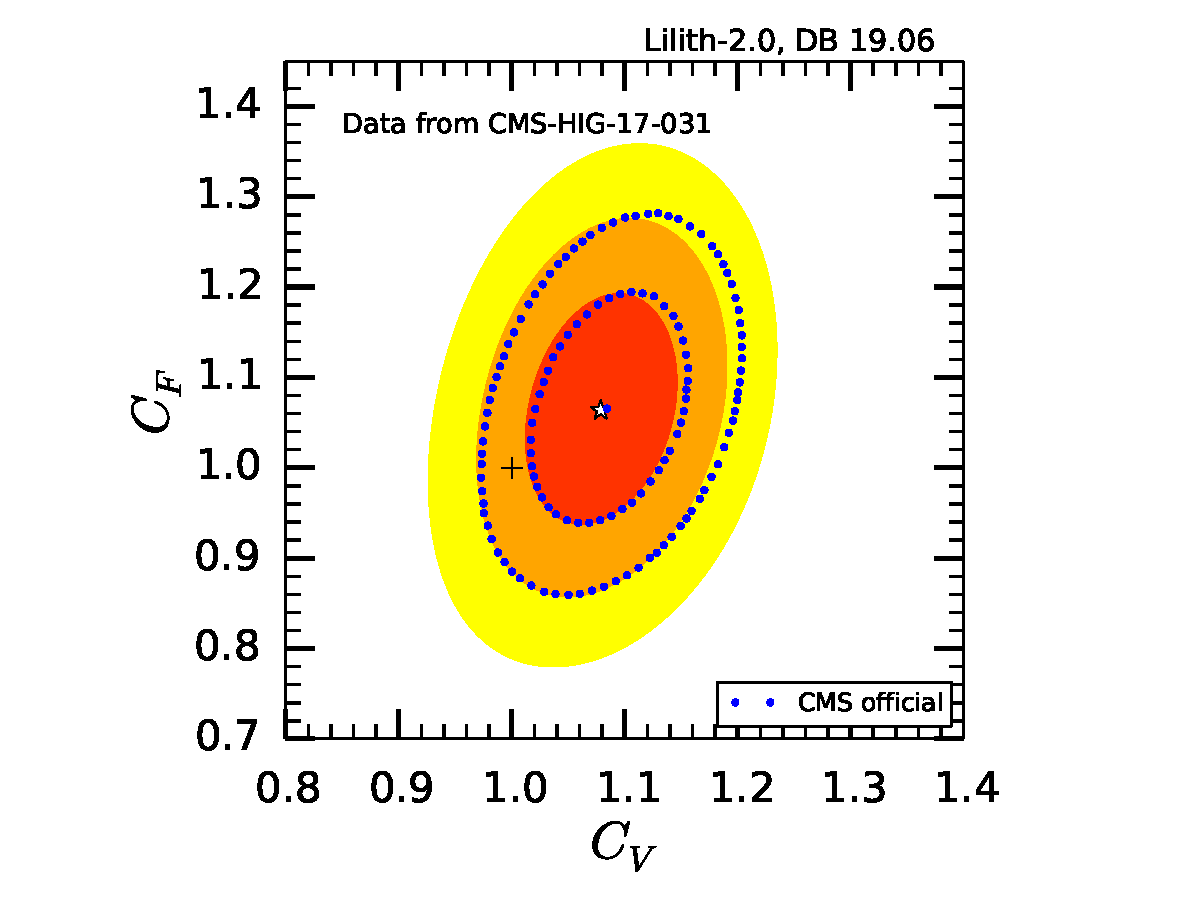
\includegraphics[width=0.5\textwidth]{validation/CMS/HIG-17-031-CVCF.pdf}
\caption{Fit of $C_F$ vs.\ $C_V$ using best-fit values and uncertainties for the signal strengths for each production (ggH, VBF, WH, ZH, ttH) 
and decay ($\gamma\gamma$, $ZZ$, $WW$, $\tau\tau$, $b\bar b$, $\mu\mu$) mode combination together with the 
$24\times 24$ correlation matrix from the CMS combination paper~\cite{Sirunyan:2018koj}. 
The  $1\sigma$,  $2\sigma$ and $3\sigma$ regions obtained with {\tt Lilith} are shown as red, orange and yellow areas, 
and compared to the $1\sigma$ and $2\sigma$ contours from CMS (blue dots).}
\label{fig:validation_cms_combination}
\end{figure}

\begin{figure}[t!]\centering
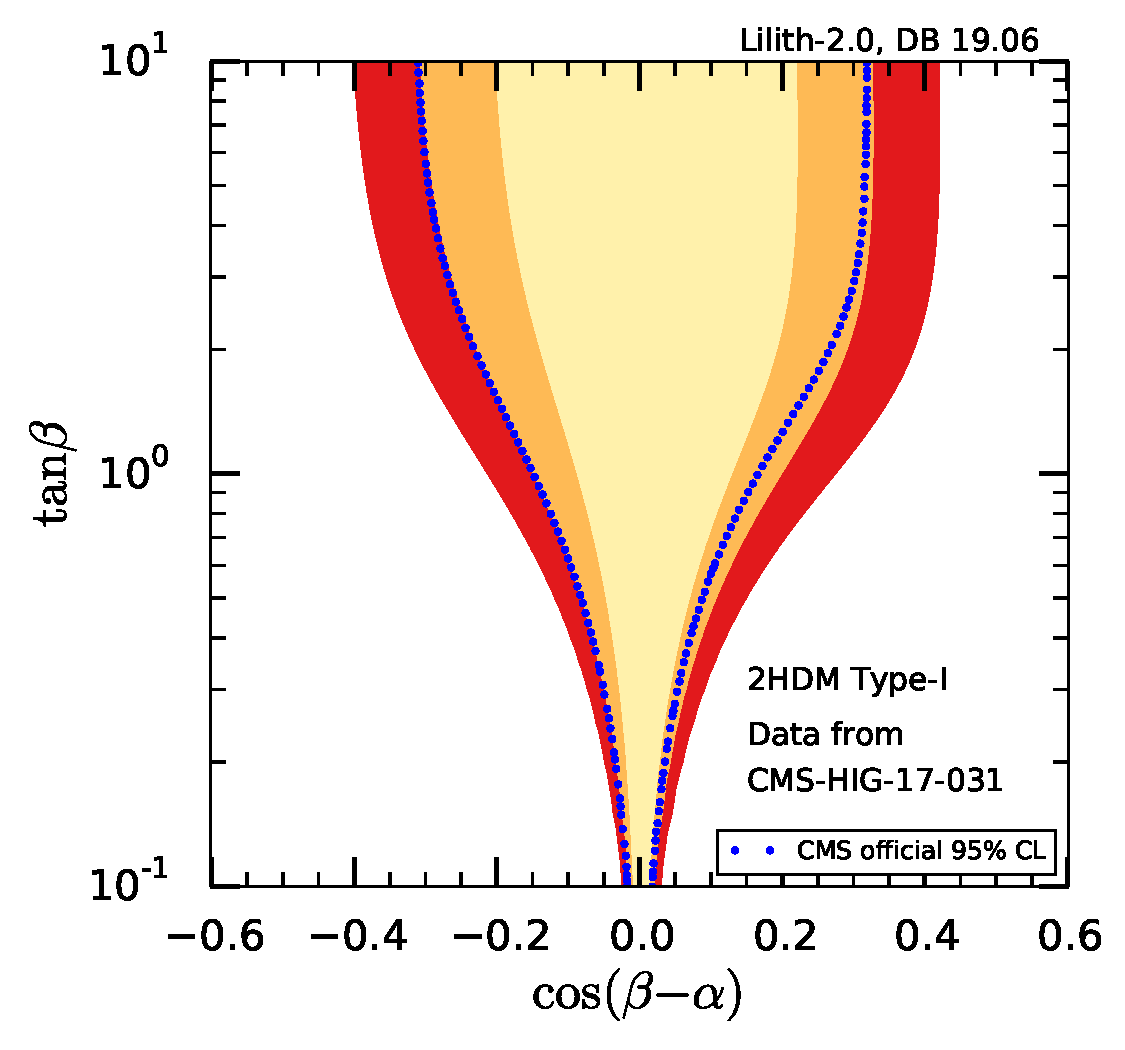
\includegraphics[width=0.4\textwidth]{validation/CMS/HIG-17-031-2HDM-Type1.pdf}%
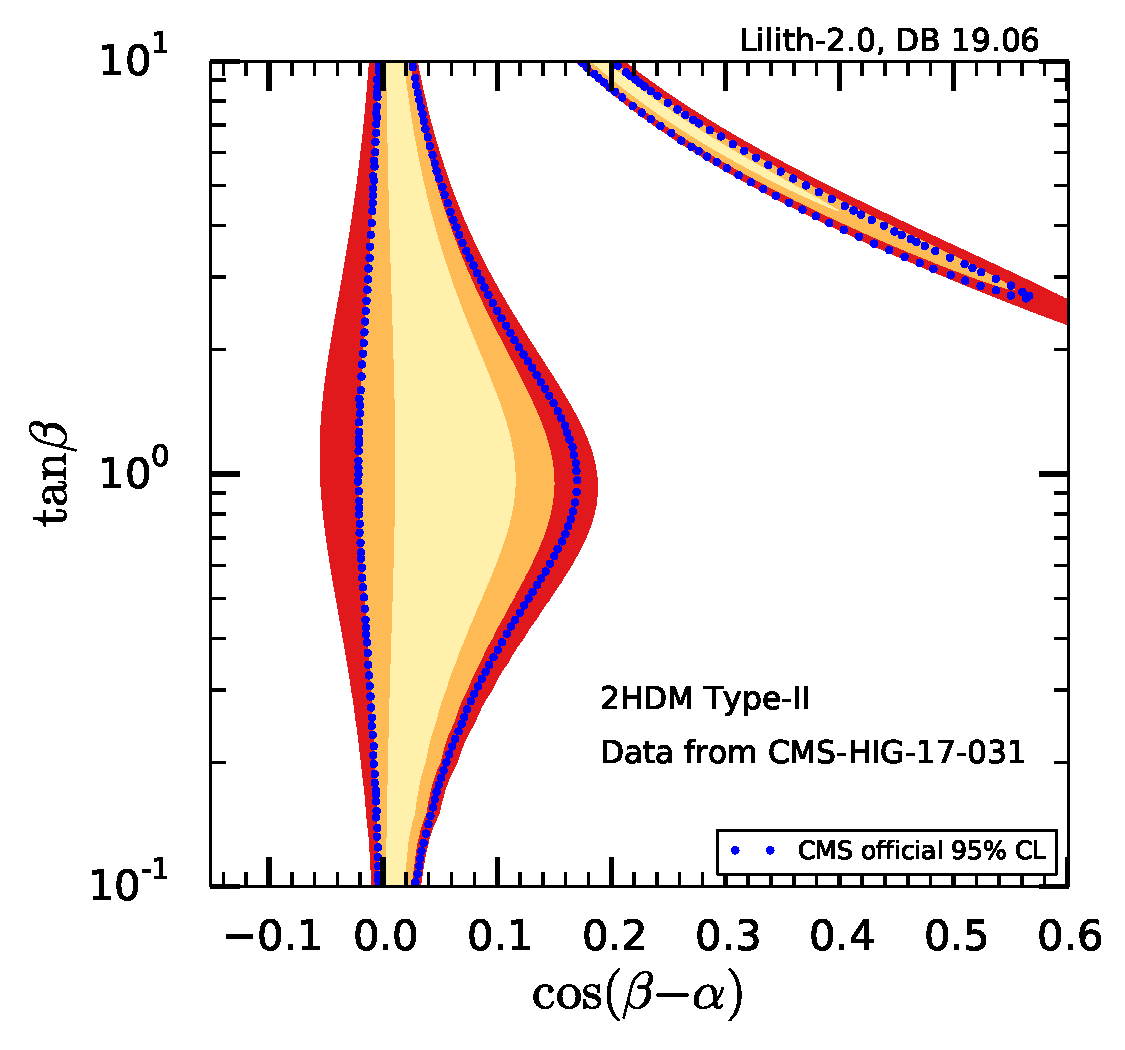
\includegraphics[width=0.4\textwidth]{validation/CMS/HIG-17-031-2HDM-Type2.pdf}
\caption{Fit of $\tan\beta$ vs.\ $\cos(\beta-\alpha)$ for the Two-Higgs-Doublet models of Type~I (left) and Type~II (right) 
using the data from the combined CMS measurement~\cite{Sirunyan:2018koj}. 
The beige, orange and red filled areas show the 68\%, 95\% and 99.7\% CL regions obtained with {\tt Lilith}, 
while the blue dots mark the 95\% CL contours from CMS.}
\label{fig:validation_cms_2hdm}
\end{figure}

{\bf\boldmath $VH$, $H\to\tau\tau$ (HIG-18-007)}: The above data from \cite{Sirunyan:2018koj} is supplemented by the results 
for the $\tau\tau$ decay mode from the $WH$ and $ZH$ targeted analysis \cite{Sirunyan:2018cpi}. These are implemented in the 
form of 1D intervals for $\mu(ZH,\;H\to\tau\tau)$ and $\mu(WH,\;H\to\tau\tau)$ taken from Fig.~6 of \cite{Sirunyan:2018cpi}. \\

{\bf\boldmath $H\to$~invisible (HIG-17-023)}: 
In \cite{Sirunyan:2018owy}, CMS performed a search for invisible decays of a Higgs boson produced through vector boson fusion. 
We use the profile likelihood ratios for the qqH-tag, Z(ll)H-, V(qq')H- and ggH-tag categories extracted 
from their Fig.~8b together with the relative contributions from the different Higgs production mechanisms  
given in Table~6 of that paper. This assumes that the relative signal contributions stay roughly the same as for 
SM production cross sections. For validation, we reproduce in Fig.~\ref{fig:validation_cms_inv}
 the $C_g$ vs.\ $C_\gamma$ fit of \cite{Sirunyan:2018koj}, where the branching ratios of invisible and undetected decays 
are treated as free parameters.%%
\footnote{The profiling in Fig.~\ref{fig:validation_cms_inv} was done with {\tt Minuit}. 
  Since {\tt Minuit} does not allow conditional limits, in this case ${\rm BR}(H\to {\rm inv.})+{\rm BR}(H\to {\rm undetected})<1$, 
  we demanded that both BR$(H\to {\rm inv.})$ and BR$(H\to {\rm undetected})$ be less than 50\%.} 

\begin{figure}[t!]\centering
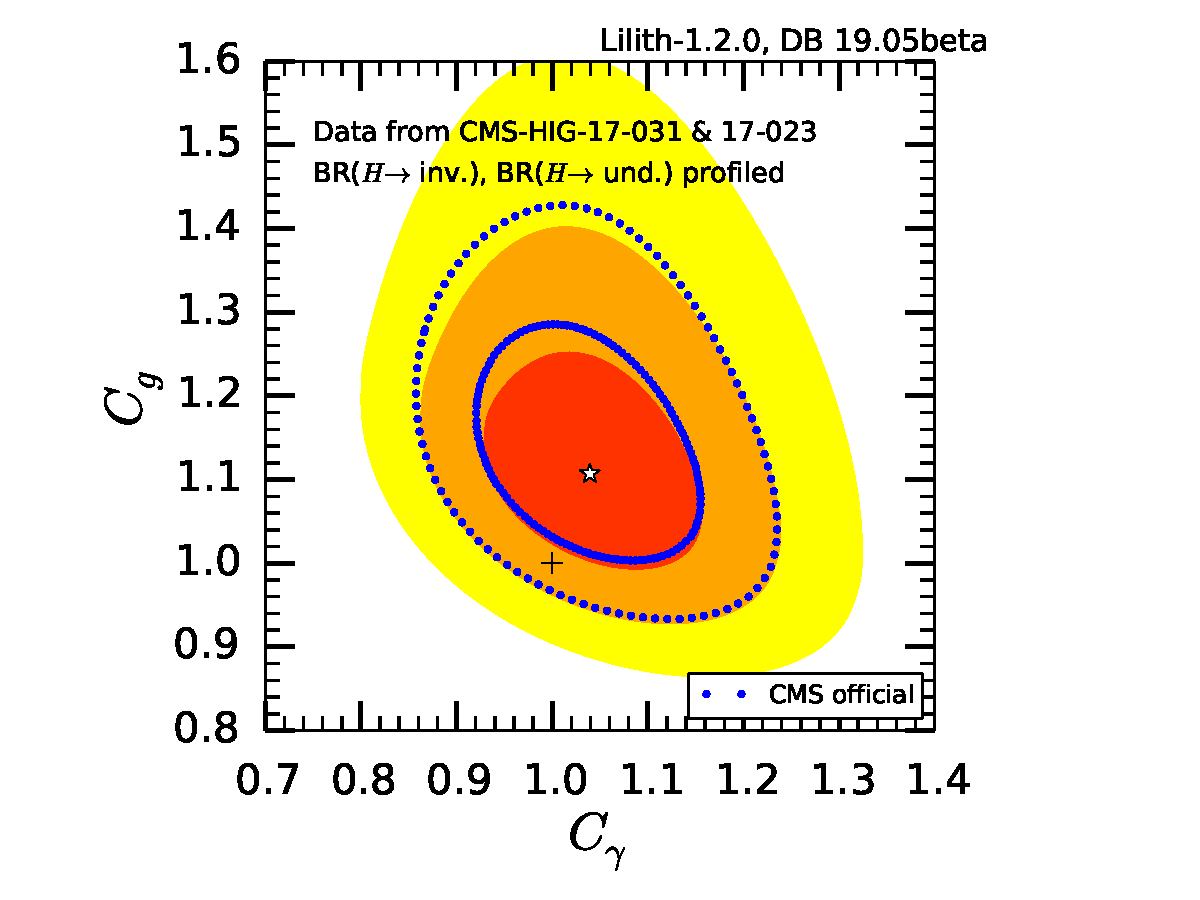
\includegraphics[width=0.5\textwidth]{validation/CMS/HIG-17-031-CgCGa_BRinvBRund_profiled.pdf}
\caption{Fit of $C_g$ vs.\ $C_\gamma$ using the data from the combined CMS measurement~\cite{Sirunyan:2018koj} and the 
search for invisible decays of a Higgs boson~\cite{Sirunyan:2018owy}. The branching ratios of invisible and undetected decays 
are treated as free parameters in the fit. 
The  $1\sigma$,  $2\sigma$ and $3\sigma$ regions obtained with {\tt Lilith} are shown as red, orange and yellow areas, 
and compared to the $1\sigma$ and $2\sigma$ contours from CMS (in blue).}
\label{fig:validation_cms_inv}
\end{figure}

